\appendix
%\begin{landscape}
\chapter{\acs{api}s}
\begin{longtable}{|c|p{56mm}|p{8cm}|}
%\textbf{\ac{api}} 	& \textbf{Member} & \textbf{Beschreibung} \kill
\caption{ARM\SymbReg Cortex\SymbReg-M \ac{api} Member und Beschreibung\label{tab:apimember}}\\
\hline

\endfirsthead
\caption[]{(Fortsetzung ARM\SymbReg Cortex\SymbReg-M \ac{api} Member und Beschreibung)}\\
\hline
\textbf{\ac{api}} 	& \textbf{Member} & \textbf{Beschreibung} \\\hline \endhead
\textbf{\ac{api}} 	& \textbf{Member} & \textbf{Beschreibung} \\\hline
\ac{spi} 			& \ttfamily{\color{blue}SPI\_API\_PTR} SPI\_API\_CREATE({\color{violet}void}) & reserviert einen Speicherbereich für die Struktur, initialisiert die Hardware des \ac{spi}, weist den Funktionspointern der Struktur die Funktionen zu und gibt die Adresse der Struktur zurück.\\\hline
\ac{spi} 			& \ttfamily {\color{violet}void} SPI\_API\_DESTROY( {\color{blue}SPI\_API\_PTR} instance) & gibt den Speicherbereich der übergebenen Struktur frei\\\hline
\ac{spi} 			& \ttfamily{\color{blue}uint32\_t} write16bit( {\color{blue}uint16\_t} *txbuff, {\color{blue}uint32\_t} transferSize) & überträgt die Daten der Adresse txbuff über den \ac{spi} an das \ac{cpld}. Die Anzahl der 16-Bit Werte wird durch den Übergabeparameter transferSize limitiert.\\\hline
\ac{spi} 			& \ttfamily{\color{blue}uint32\_t} transfer16bit( {\color{blue}uint16\_t} *txbuff, {\color{blue}uint16\_t} *rxbuff, {\color{blue}uint32\_t} transferSize) & siehe write16bit, hinzu kommt, dass die Daten des \ac{spi}-Slaves in die Adresse rxbuff und folgend geschrieben werden.\\\hline
\ac{usb} 			& \ttfamily{\color{blue}USB\_API\_PTR} USB\_API\_CREATE({\color{violet}void}) & reserviert einen Speicherbereich für die Struktur, weist den Descriptoren der \ac{usb} Register die applikationsspezifischen Descriptoren zu, registriert die Endpunkte, initialisiert die Hardware der \ac{usb} 2.0 Schnittstelle und gibt die Adresse der Struktur zurück.\\\hline
\ac{usb} 			& \ttfamily {\color{violet}void} USB\_API\_DESTROY( {\color{blue}USB\_API\_PTR} instance) & gibt den Speicherbereich der übergebenen Struktur frei\\\hline
\ac{usb} 			& \ttfamily {\color{violet}extern} {\color{violet}void} PerformUSB\_Vendor({\color{blue}uint8\_t} cmd, {\color{blue}uint16\_t} Value) & Funktion, welche in der Applikation implementiert werden muss. Diese Funktion kann genutzt werden, um die Befehle des Nutzers und dessen Parameter auszulesen. \\\hline

SCT 				& \ttfamily {\color{violet}extern volatile} {\color{blue}uint8\_t} buffer[16384] & Speicherbereich für 4096 32-Bit Werte\\\hline
SCT 				& \ttfamily {\color{violet}typedef enum} {\color{blue}TransferType} & Enumeration für die Unterscheidung der Datenpakete (RF Daten, Basis oder erstes harmonisch demoduliertes Datenpaket)\\\hline
SCT 				& \ttfamily {\color{violet}void} USD\_HW\_DATAPORT\_CREATE( {\color{violet}void}(*ROI\_dataReceived) ({\color{blue}TransferType} dataType)) & Weist der Callback Funktion den übergebenen Funktionspointer zu. \\\hline
SCT 				& \ttfamily {\color{violet}void} USD\_HW\_DATAPORT\_START( {\color{violet}void}) & Parametriert die Hardware Pins, initialisiert den \ac{dma}-Controller und den SCT. \\\hline

USD 				& \ttfamily{\color{blue}USD\_HW\_VALUES} Config & Struktur, welche die Einstellungen des \ac{cpld}s beinhaltet. \\\hline
%USD 				& \ttfamily{\color{blue}uint8\_t} Mode & \\\hline
USD 				& \ttfamily {\color{violet}void} ResetUSD({\color{violet}void}) & Funktion, welche das \ac{cpld} in einen definierten Zustand bringt.\\\hline
USD 				& \ttfamily {\color{violet}void} WriteConfig({\color{violet}void}) & Funktion, welche die Einstellung in das \ac{cpld} via \ac{spi} schreibt. \\\hline
USD 				& \ttfamily {\color{violet}void} ReadConfig({\color{blue}uint16\_t*} data) & Funktion, welche die Register des \ac{cpld}s liest und in den Übergabeparameter data schreibt.\\\hline
USD 				& \ttfamily {\color{violet}void} Start({\color{violet}void}) & Startet den Zustandsautomaten des \ac{cpld}s \\\hline
USD 				& \ttfamily {\color{violet}void} Stop({\color{violet}void}) & Stoppt den Zustandsautomaten des \ac{cpld}s\\\hline
USD 				& \ttfamily {\color{violet}extern} {\color{blue}USD\_HW\_API\_PTR} usdhandle & Strukturpointer, welcher die Einstellungen und die Funktionen für das \ac{cpld} beinhaltet. \\\hline
USD 				& \ttfamily {\color{blue}USD\_HW\_API\_PTR} USD\_HW\_API\_CREATE({\color{violet}void}) & reserviert einen Speicherbereich für die Struktur, weist der Konfiguration und den Funktionspointern Einstellungen und Funktionen zu, initialisiert die benötigte Hardware und gibt die Adresse der Struktur zurück.\\\hline
USD 				& \ttfamily {\color{violet}void} USD\_HW\_API\_DESTROY( {\color{blue}USD\_HW\_API\_PTR}) & gibt den Speicherbereich der übergebenen Struktur frei\\\hline
\end{longtable}

\chapter{Testergebnisse}
\section{Impedanz-Frequenzdiagramme der vorhandenen Sonden}\label{sec:sonden}
%\lstinputlisting[caption=Matlab \ac{snr} Test Skript, escapechar=, label=lst:matlab_snr, style=Matlab]{sourcecode/Test_SNR.m}
\begin{figure}[ht!]
	\centering
	\begin{subfigure}[t!]{0.82\textwidth}
		\centering
  		\includegraphics[page=1,width=\textwidth, trim= 31mm 178mm 36mm 22mm, clip=true]{attachment/Impedanzen_Sonden.pdf}% \\[.5cm]
 		\caption{Messung mit Gel auf der Hand}
 		\label{fig:2_sig}
  	\end{subfigure}
  	\begin{subfigure}[t!]{0.82\textwidth}
	  	\centering
  		\includegraphics[page=1,width=\textwidth, trim= 26mm 40mm 36mm 160mm, clip=true]{attachment/Impedanzen_Sonden.pdf} %\\[.5cm]
  		\caption{Messung an der Luft}
 		\label{fig:snr_2_script}
  	\end{subfigure}
  	\caption{2 \acs{mhz} Feroperm Piezoelement mit Kupferhülse und geklebter Linse}
\end{figure}
\clearpage

\begin{figure}[ht!]
	\centering
	\begin{subfigure}[t!]{0.82\textwidth}
	  	\centering
  		\includegraphics[page=3,width=\textwidth, trim= 27mm 63mm 37mm 137mm, clip=true]{attachment/Impedanzen_Sonden.pdf} %\\[.5cm]
  		\caption{normal}
 		\label{fig:snr_2_script}
  	\end{subfigure}
  	\begin{subfigure}[t!]{0.82\textwidth}
	  	\centering
  		\includegraphics[page=5,width=\textwidth, trim= 26mm 64mm 37mm 137mm, clip=true]{attachment/Impedanzen_Sonden.pdf} %\\[.5cm]
  		\caption{im Kupferring}
 		\label{fig:snr_2_script}
  	\end{subfigure}
  	\caption{2 \acs{mhz} Kristall an der Luft}
\end{figure}
\clearpage

\begin{figure}[ht!]
	\centering
	\begin{subfigure}[t!]{0.82\textwidth}
	  	\centering
  		\includegraphics[page=6,width=\textwidth, trim= 28mm 178mm 39mm 22mm, clip=true]{attachment/Impedanzen_Sonden.pdf} %\\[.5cm]
  		\caption{Messung mit Gel auf der Hand}
 		\label{fig:snr_2_script}
  	\end{subfigure}
  	\begin{subfigure}[t!]{0.82\textwidth}
	  	\centering
  		\includegraphics[page=6,width=\textwidth, trim= 32mm 42mm 39mm 158mm, clip=true]{attachment/Impedanzen_Sonden.pdf} %\\[.5cm]
  		\caption{Messung an der Luft}
 		\label{fig:snr_2_script}
  	\end{subfigure}
  	\caption{2,25 \acs{mhz} Feroperm Piezoelement mit Kupferhülse und geklebter Linse}
\end{figure}
\clearpage

\begin{figure}[ht!]
	\centering
	\begin{subfigure}[t!]{0.82\textwidth}
	  	\centering
  		\includegraphics[page=8,width=\textwidth, trim= 26mm 170mm 47mm 30mm, clip=true]{attachment/Impedanzen_Sonden.pdf} %\\[.5cm]
  		\caption{schwarz}
 		\label{fig:snr_2_script}
  	\end{subfigure}
  	\begin{subfigure}[t!]{0.82\textwidth}
	  	\centering
  		\includegraphics[page=8,width=\textwidth, trim= 38mm 55mm 47mm 144mm, clip=true]{attachment/Impedanzen_Sonden.pdf} %\\[.5cm]
  		\caption{weiß}
 		\label{fig:snr_2_script}
  	\end{subfigure}
  	\caption{4 \acs{mhz} Hollerith Sonde}
\end{figure}
\clearpage


\begin{figure}[ht!]
	\centering
	\begin{subfigure}[t!]{0.82\textwidth}
	  	\centering
  		\includegraphics[page=10,width=\textwidth, trim= 39mm 64mm 47mm 136mm, clip=true]{attachment/Impedanzen_Sonden.pdf} %\\[.5cm]
  		\caption{schwarz}
 		\label{fig:snr_2_script}
  	\end{subfigure}
  	\begin{subfigure}[t!]{0.82\textwidth}
	  	\centering
  		\includegraphics[page=10,width=\textwidth, trim= 39mm 178mm 47mm 22mm, clip=true]{attachment/Impedanzen_Sonden.pdf} %\\[.5cm]
  		\caption{weiß}
 		\label{fig:snr_2_script}
  	\end{subfigure}
  	\caption{8 \acs{mhz} Hollerith Sonde}
\end{figure}
\clearpage
%\end{landscape}
\section{Signalintensitätsmessung auf Übersprechen mit Nahfeldsonde}\label{sec:signal_db}
\begin{figure}[h!]
  \centering
  \begin{subfigure}[t]{0.48\textwidth}
	\centering
  	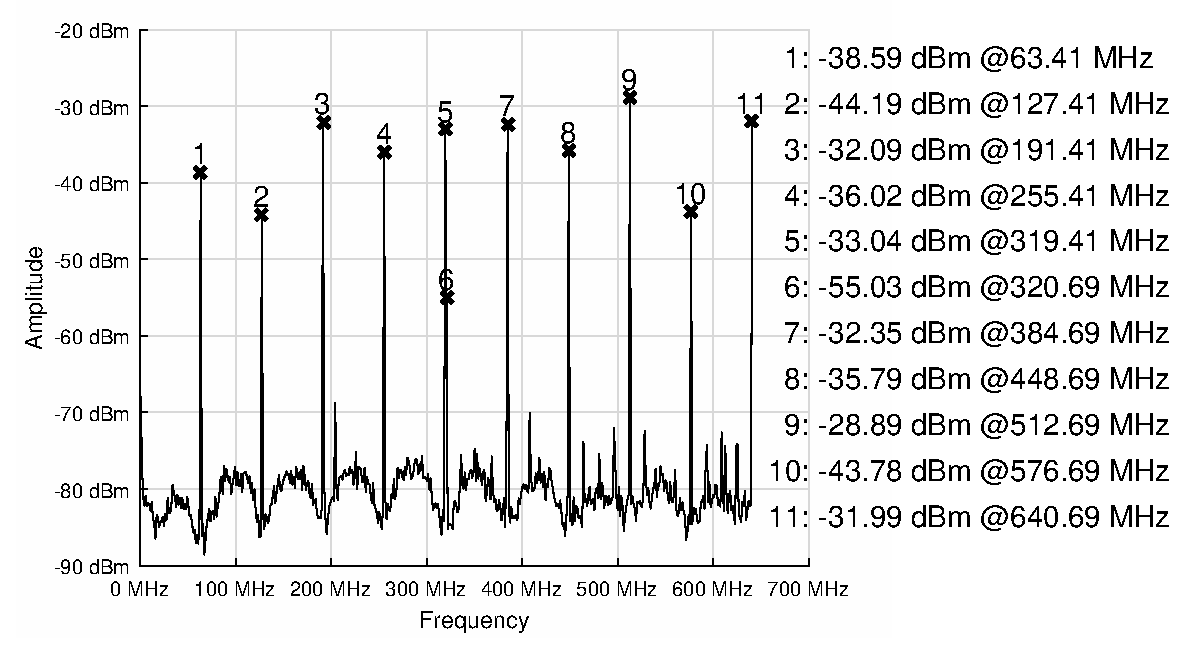
\includegraphics[width=\textwidth]{tests/sonde/m1.eps}  
  	\caption{Oberseite - Sonde über geschildeter \ac{adc} Taktleitung}
  	\label{fig:m1}
  \end{subfigure}
  ~
  \begin{subfigure}[t]{0.48\textwidth}
	\centering
  	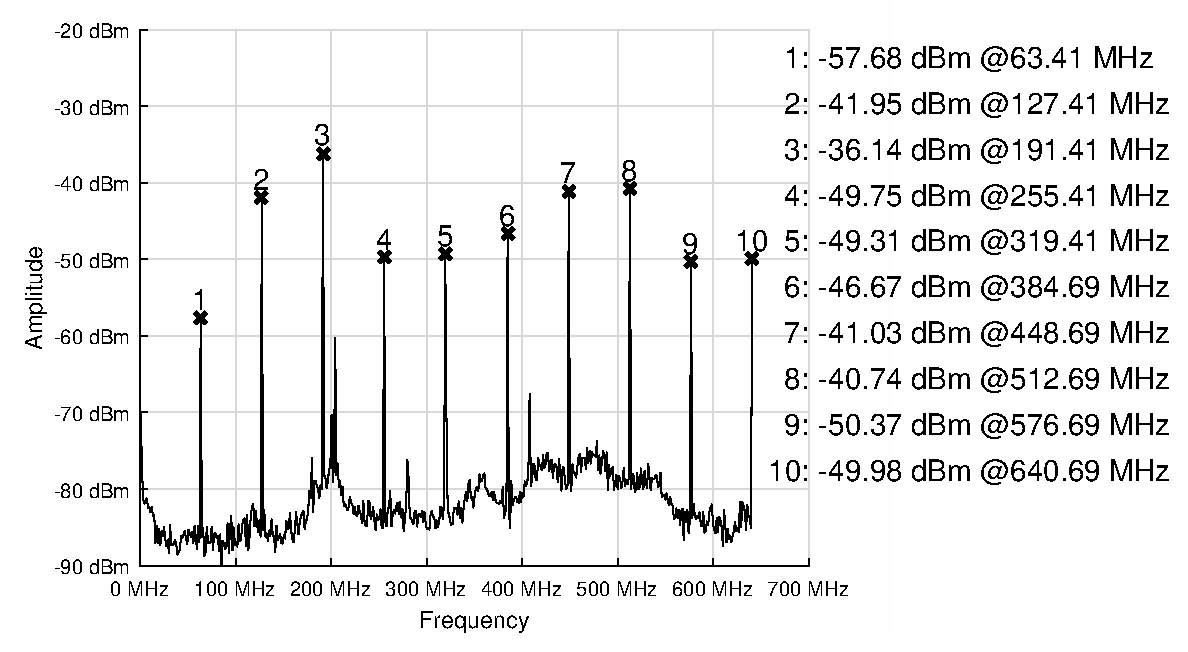
\includegraphics[width=\textwidth]{tests/sonde/m1_001.eps}  
  \caption{Oberseite - Sonde über Schild-Massefläche nahe \ac{adc}}
  \label{fig:m2}
  \end{subfigure}
  ~
  \begin{subfigure}[t]{0.48\textwidth}
	\centering
  	\includegraphics[width=\textwidth]{tests/sonde/m1_002.eps}  
  	  \caption{Oberseite - Sonde über digitaler Massefläche zwischen \ac{adc}-Datenleitungen}
  \label{fig:m2}
  \end{subfigure}
  ~
  \begin{subfigure}[t]{0.48\textwidth}
	\centering
  	\includegraphics[width=\textwidth]{tests/sonde/m1_003.eps}  
  	\caption{Oberseite - Sonde über analoger Massefläche bei Bandpass}
  \label{fig:m2}
  \end{subfigure}
  ~
  \begin{subfigure}[t]{0.48\textwidth}
	\centering
  	\includegraphics[width=\textwidth]{tests/sonde/m1_004.eps}  
  	\caption{Oberseite - Sonde über Schild-Massefläche nahe Bandpass}
  \label{fig:m2}
  \end{subfigure}
  ~
  \begin{subfigure}[t]{0.48\textwidth}
	\centering
  	\includegraphics[width=\textwidth]{tests/sonde/m1_007.eps}  
  	\caption{Oberseite - Sonde über Schild-Massefläche nahe Bandpass 90$^\circ$ gedreht}
  \label{fig:m2}
  \end{subfigure}
  ~
  \begin{subfigure}[t]{0.48\textwidth}
	\centering
  	\includegraphics[width=\textwidth]{tests/sonde/m1_006.eps}  
  	\caption{Oberseite - Sonde an linker oberer Ecke des LPC4337}
  \label{fig:m2}
  \end{subfigure}
  ~
  \begin{subfigure}[t]{0.48\textwidth}
	\centering
  	\includegraphics[width=\textwidth]{tests/sonde/m1_005.eps}  
  	\caption{Oberseite - Sonde über digitaler Masserfläche zwischen Antiparallelen Dioden D3 und U3}
  \label{fig:m2}
  \end{subfigure}
\end{figure}
\clearpage
\begin{figure}[h!]
\ContinuedFloat
        \centering
  \begin{subfigure}[t]{0.48\textwidth}
	\centering
  	\includegraphics[width=\textwidth]{tests/sonde/m1_008.eps}  
  	\caption{Oberseite - Sonde nach Vorverstärker unterhalb der Testpunkte}
  \label{fig:m2}
  \end{subfigure}
  ~
  \begin{subfigure}[t]{0.48\textwidth}
	\centering
  	\includegraphics[width=\textwidth]{tests/sonde/m1_009.eps}  
  	\caption{Oberseite - Sonde nach Vorverstärker oberhalb der Testpunkte}
  \label{fig:m2}
  \end{subfigure}
  ~
  \begin{subfigure}[t]{0.48\textwidth}
	\centering
  	\includegraphics[width=\textwidth]{tests/sonde/m1_010.eps}  
  	\caption{Oberseite - Sonde oberhalb des rechten \ac{adc}-Eingangs}
  \label{fig:m2}
  \end{subfigure}
  ~
  \begin{subfigure}[t]{0.48\textwidth}
	\centering
  	\includegraphics[width=\textwidth]{tests/sonde/m1_011.eps}  
  	\caption{Oberseite - Sonde an unterer linker Ecke des \ac{adc} (analoge Seite)}
  \label{fig:m2}
  \end{subfigure}
  ~
  \begin{subfigure}[t]{0.48\textwidth}
	\centering
  	\includegraphics[width=\textwidth]{tests/sonde/m1_012.eps}  
  	\caption{Oberseite - Sonde an oberer linker Ecke des \ac{adc} (analoge Seite)}
  \label{fig:m2}
  \end{subfigure}
  ~
  \begin{subfigure}[t]{0.48\textwidth}
	\centering
  	\includegraphics[width=\textwidth]{tests/sonde/m1_013.eps}  
  	\caption{Oberseite - Sonde an oberer rechten Ecke des \ac{adc} (digitale Seite)}
  \label{fig:m2}
  \end{subfigure}
  ~
  \begin{subfigure}[t]{0.48\textwidth}
	\centering
  	\includegraphics[width=\textwidth]{tests/sonde/m1_014.eps}  
  	\caption{Oberseite - Sonde an \ac{lna} vor Ferrit}
  \label{fig:m2}
  \end{subfigure}
  ~
  \begin{subfigure}[t]{0.48\textwidth}
	\centering
  	\includegraphics[width=\textwidth]{tests/sonde/m1_015.eps}  
  	\caption{Oberseite - Sonde an \ac{lna} nach Ferrit}
  \label{fig:m2}
  \end{subfigure}
\end{figure}
\clearpage
\begin{figure}[h!]
\ContinuedFloat
        \centering
  \begin{subfigure}[t]{0.48\textwidth}
	\centering
  	\includegraphics[width=\textwidth]{tests/sonde/m1_016.eps}  
  	\caption{Unterseite - Sonde an 64 \ac{mhz} Oszillatorausgang}
  \label{fig:m2}
  \end{subfigure}
  ~
  \begin{subfigure}[t]{0.48\textwidth}
	\centering
  	\includegraphics[width=\textwidth]{tests/sonde/m1_017.eps}  
  	\caption{Unterseite - Sonde bei \ac{adc} Stützelkos}
  \label{fig:m2}
  \end{subfigure}
  ~
  \begin{subfigure}[t]{0.48\textwidth}
	\centering
  	\includegraphics[width=\textwidth]{tests/sonde/m1_018.eps}  
  	\caption{Unterseite - Sonde bei Sondenanschluss}
  \label{fig:m2}
  \end{subfigure}
	~
  \begin{subfigure}[t]{0.48\textwidth}
	\centering
  	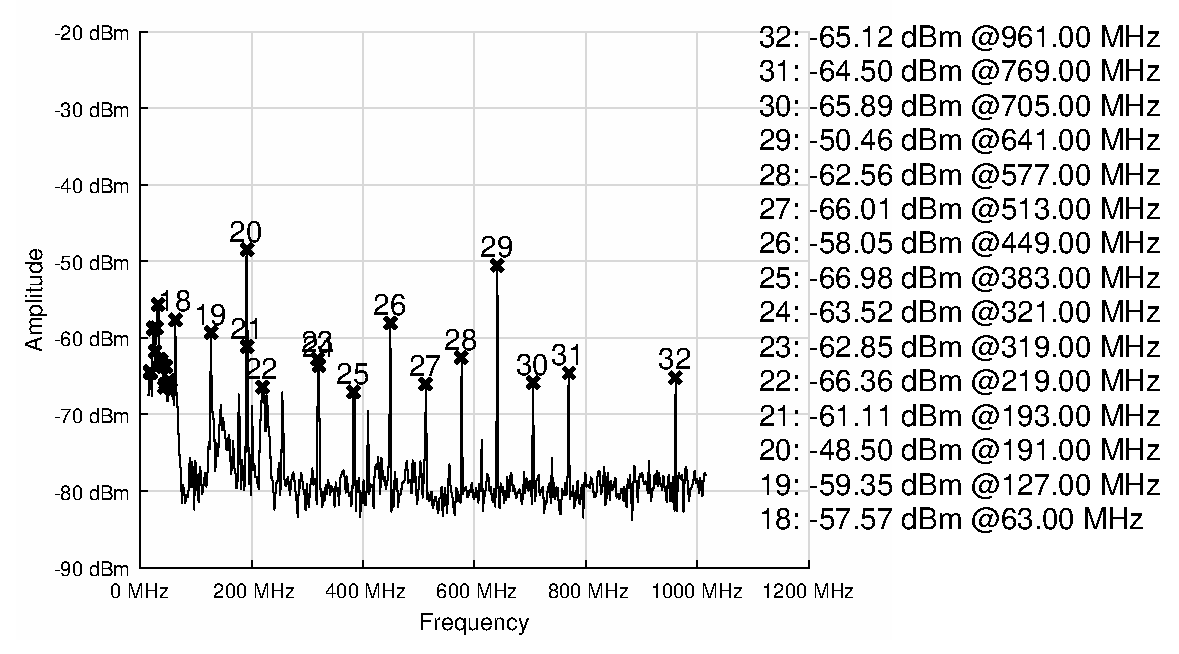
\includegraphics[width=\textwidth]{tests/sonde/ringkern_Sonde.eps}  
  	\caption{Stromzange an Signalausgang zur Sonde}
  \label{fig:strom_sonde}
  \end{subfigure}
  ~
  \begin{subfigure}[t]{0.48\textwidth}
	\centering
  	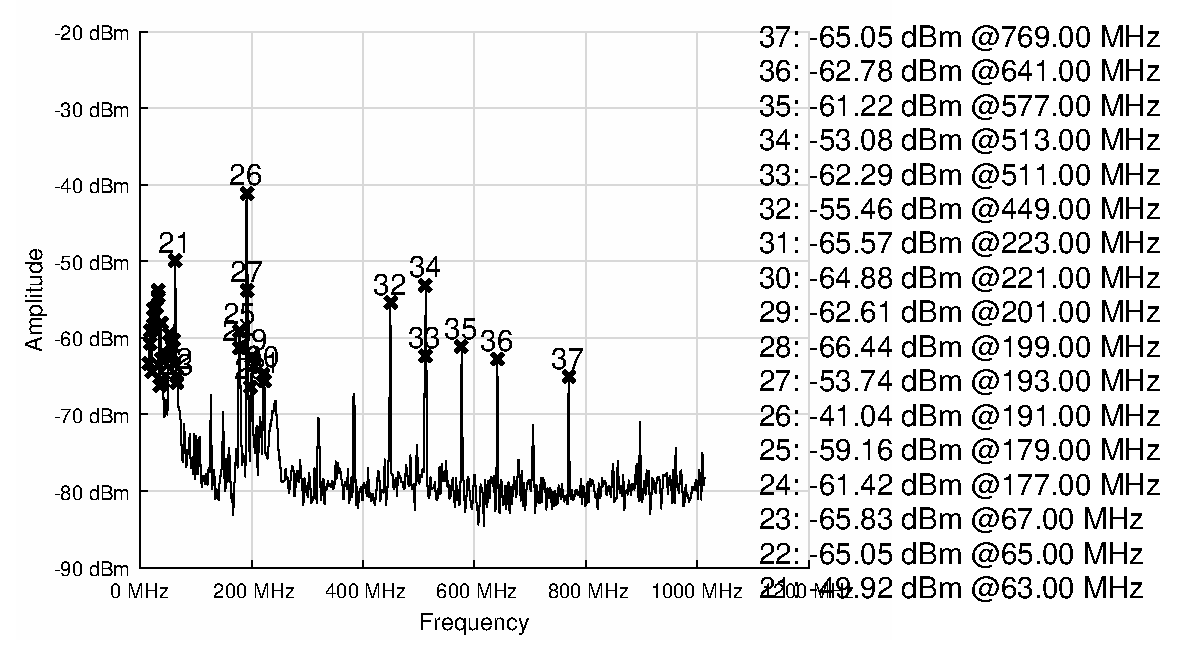
\includegraphics[width=\textwidth]{tests/sonde/ringkern_Spannung.eps}  
  	\caption{Stromzange um \acs{pc} \acs{usb}-Kabel}
  \label{fig:strom_spannung}
  \end{subfigure}  
  \caption{Signalintegrität}
  \label{fig:signal_int}
\end{figure}
\clearpage
\chapter{Dokumente}
\begin{center}
\begin{tabular}{|p{12cm}|c|}
\hline 
Beschreibung & Link zu Anhang \\ 
\hline 
Schaltplan Version 1.1 & \attachfile[icon=Paperclip]{images/pcb/USD2015_0101.pdf}  \\
3D Layout & \attachfile[icon=Paperclip]{attachment/USD2015.pdf}  \\
%Datenblatt Rail-to-Rail xDSL Verstärker AD8018 & \attachfile[icon=Paperclip]{attachment/Datenblaetter/AD8018.pdf}  \\
%Datenblatt differenzieller Operationsverstärker AD8351 & \attachfile[icon=Paperclip]{attachment/Datenblaetter/AD8351.pdf}  \\
%Datenblatt \ac{adc} AD9245 & \attachfile[icon=Paperclip]{attachment/Datenblaetter/AD9245.pdf}  \\
%Datenblatt MachXO & \attachfile[icon=Paperclip]{attachment/Datenblaetter/MachXO.pdf}  \\
%LT-Spice Bandpass & \attachfile[icon=Paperclip]{attachment/LTSpice_Eingangsfilter.asc}  \\
%Thesis - Stempelwitz Sebastian & \attachfile[icon=Paperclip]{attachment/Thesis-Stemplewitz.pdf}  \\
%Thesis - Rehn, Andreas & \attachfile[icon=Paperclip]{attachment/Thesis-Rehn.pdf}  \\
\hline 
%2 \ac{mhz} Signal bei 320 mV Eingangssignal gemessen mit 64 \ac{mhz} & \attachfile[icon=Paperclip]{attachment/SNR/64-2-0.32.txt}  \\
%4 \ac{mhz} Signal bei 320 mV Eingangssignal gemessen mit 64 \ac{mhz} & \attachfile[icon=Paperclip]{attachment/SNR/64-4-0.32.txt}  \\
%6 \ac{mhz} Signal bei 320 mV Eingangssignal gemessen mit 64 \ac{mhz} & \attachfile[icon=Paperclip]{attachment/SNR/64-6-0.32.txt}  \\
%8 \ac{mhz} Signal bei 320 mV Eingangssignal gemessen mit 64 \ac{mhz} & \attachfile[icon=Paperclip]{attachment/SNR/64-8-0.32.txt}  \\
%Matlab - digitaler Hochpass Filter Fixed Point (Skript) & \attachfile[icon=Paperclip]{attachment/SNR/perfect.m}  \\
%Matlab - Kalkulation mit Visualisierung der gemessenen Signale (Skript) & \attachfile[icon=Paperclip]{attachment/SNR/Test_SNR.m}  \\
\hline 
\end{tabular}
\end{center}
\chapter{Schaltplan und Layout}
\section{Schaltplan}
%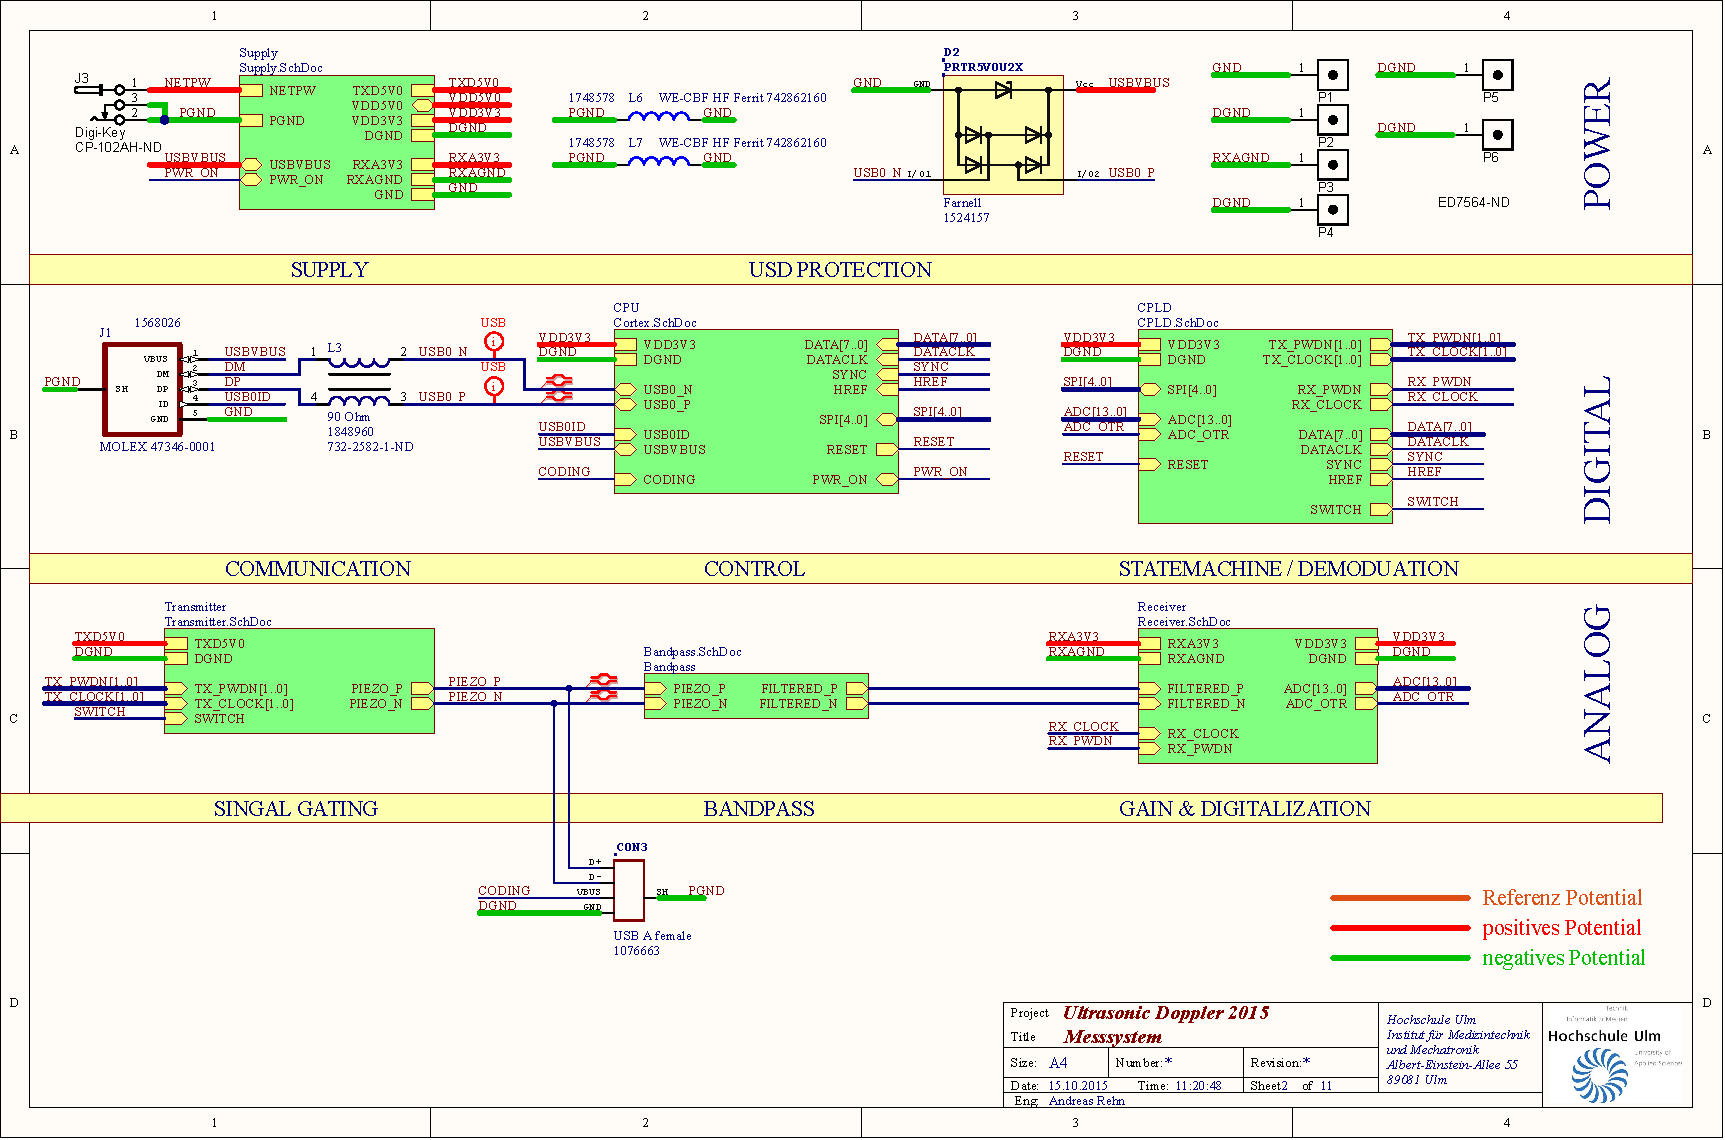
\includepdf[pages=-,landscape=true]{images/pcb/USD2015_0101.pdf}
\section{Layout}
%\includepdf[pages=1-5]{attachment/USD2015-docu1.pdf}